\talkslide{beam-benchmarks}{Beam: benchmark results}{Timing: provisional}{Survey the report's 22 benchmarks, preserving the original overview.}{
\centering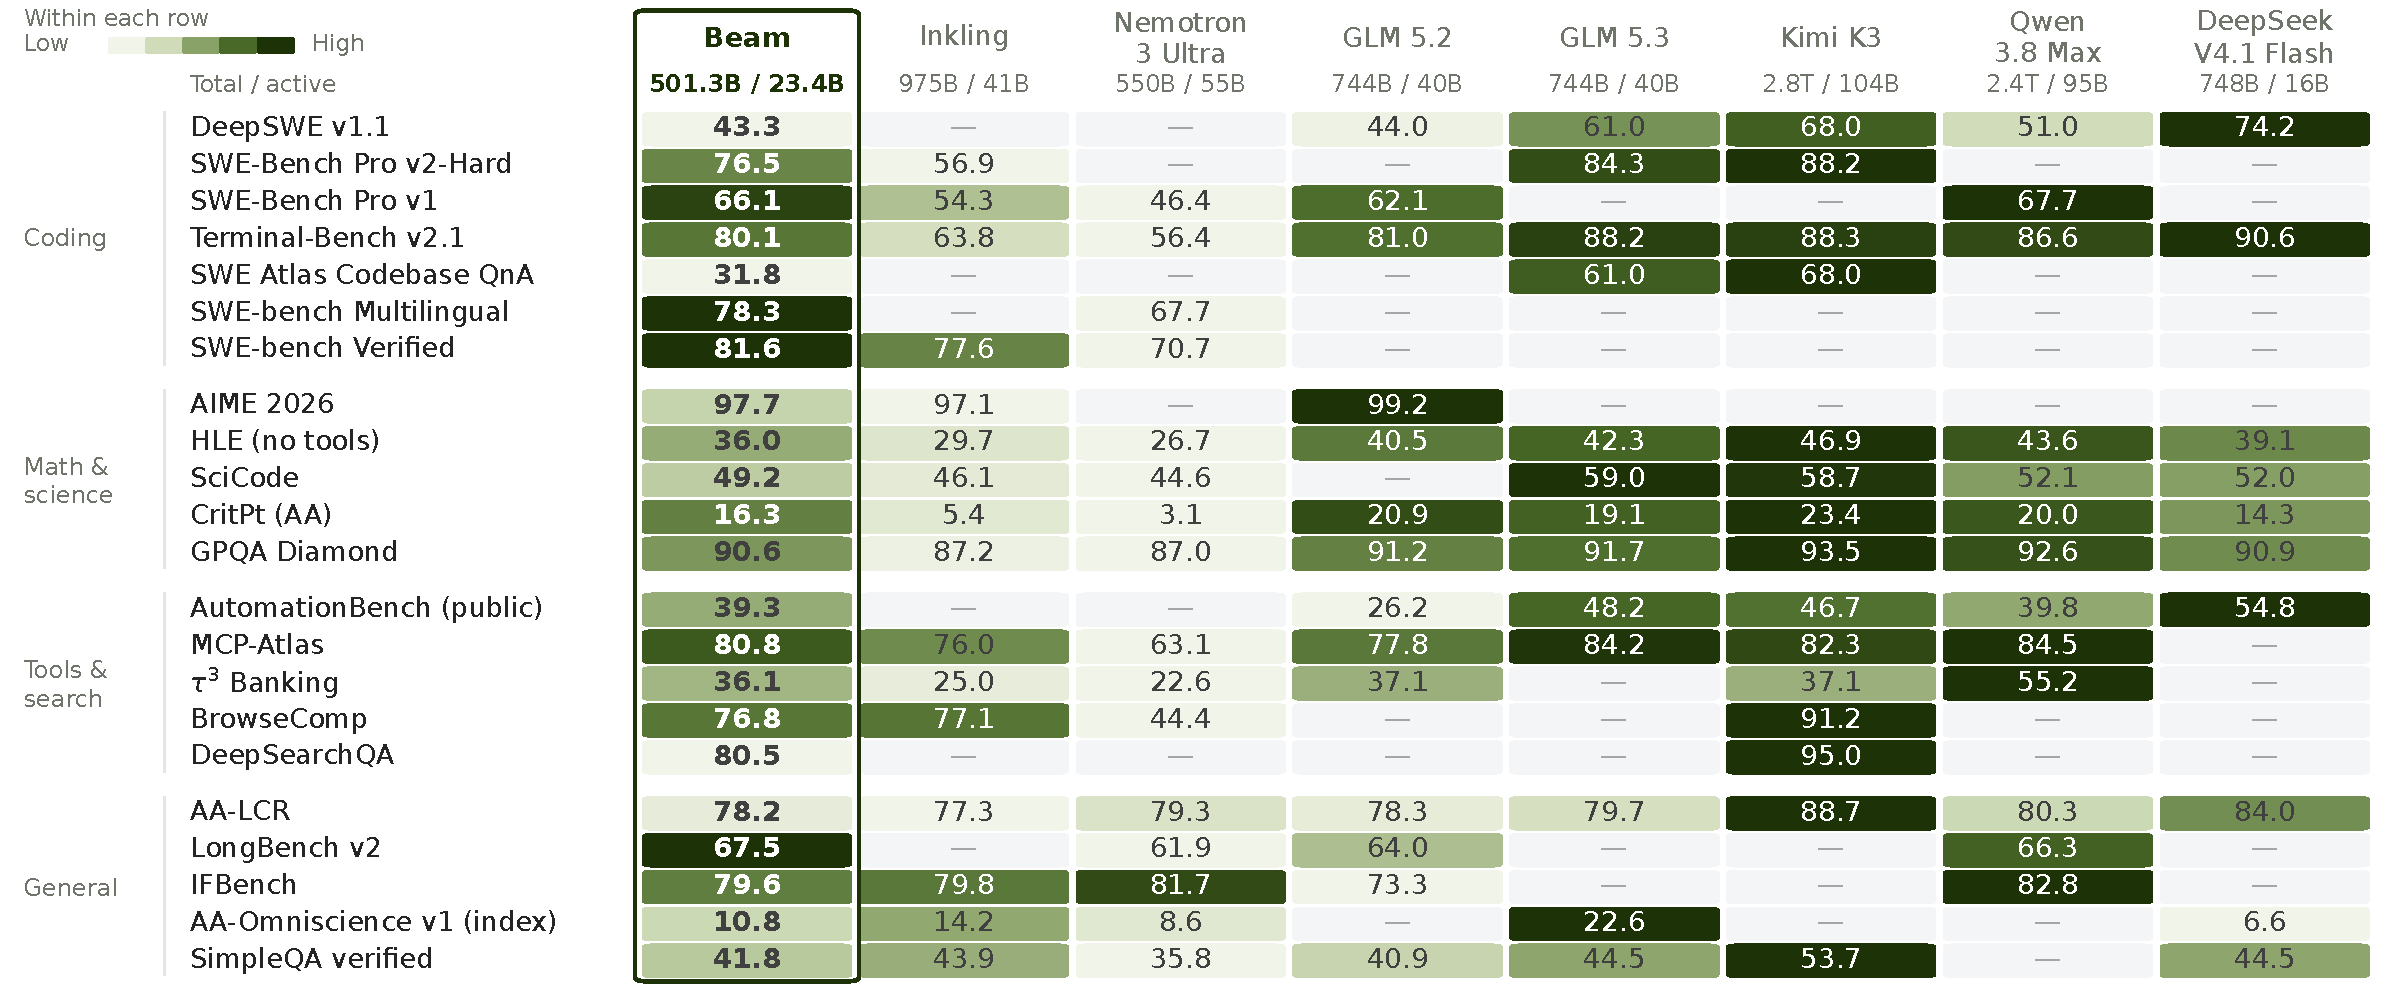
\includegraphics[width=\linewidth,height=6.5cm,keepaspectratio]{assets/beam-intro/benchmark-summary.pdf}
}
\speak{This is the full benchmark overview copied from the Beam presentation. It covers coding, mathematics and science, tool use and search, and general capabilities. Beam is highlighted, and darker cells indicate higher scores within each row. The headers give total and active parameters, with B for billions and T for trillions beside each value. AA-Omniscience is an index; the other scores are percentages. BrowseComp and DeepSearchQA use context management, and DeepSeek's active parameter count is for decoding. This is the report's comparison snapshot, not an updated leaderboard. The source figure is copied without changing its data or model set. Source: Beam technical report, the four post-training comparison tables; Beam presentation, Benchmarks slide and figures/evaluations.json.}
